\documentclass[12pt]{beamer}
\newenvironment{ConCodigo}[1]
  {\begin{frame}[fragile,environment=ConCodigo]{#1}}
  {\end{frame}}
\graphicspath{{Imagenes/}{../Imagenes/}}
\usepackage[utf8]{inputenc}
\usepackage[spanish]{babel}
\usepackage{hyperref}
\usepackage{etex}
\reserveinserts{28}
\usepackage{amsmath}
\usepackage{amsthm}
\usepackage{mathtools}
\usepackage{multicol}
\usepackage{multirow}
\usepackage{tabulary}
%\usepackage{tabularx}
\usepackage{booktabs}
\usepackage{nccmath}
\usepackage{biblatex}
\usepackage{epstopdf}
\usepackage{graphicx}
\usepackage{siunitx}
\sisetup{scientific-notation=true}
%\usepackage{fontspec}
\usepackage{lmodern}
\usepackage{float}
\usepackage[format=hang, font=footnotesize, labelformat=parens]{caption}
\usepackage[autostyle,spanish=mexican]{csquotes}
\usepackage{standalone}
\usepackage{tikz}
\usepackage[siunitx]{circuitikz}
\usetikzlibrary{arrows,patterns,shapes}
\usetikzlibrary{decorations.markings}
\usetikzlibrary{arrows}
\usepackage{color}
%\usepackage{beton}
%\usepackage{euler}
%\usepackage[T1]{fontenc}
\usepackage[sfdefault]{roboto}  %% Option 'sfdefault' only if the base font of the document is to be sans serif
\usepackage[T1]{fontenc}
\renewcommand*\familydefault{\sfdefault}
\DeclareGraphicsExtensions{.pdf,.png,.jpg}
\usepackage{hyperref}
\renewcommand {\arraystretch}{1.5}
\newcommand{\python}{\texttt{python}}
\usefonttheme[onlymath]{serif}
\setbeamertemplate{navigation symbols}{}
\usetikzlibrary{patterns}
\usetikzlibrary{decorations.markings}
\tikzstyle{every picture}+=[remember picture,baseline]
%\tikzstyle{every node}+=[inner sep=0pt,anchor=base,
%minimum width=2.2cm,align=center,text depth=.15ex,outer sep=1.5pt]
%\tikzstyle{every path}+=[thick, rounded corners]
\setbeamertemplate{caption}[numbered]
\newcommand{\ptm}{\fontfamily{ptm}\selectfont}
%Se usa la plantilla Warsaw modificada con spruce
\mode<presentation>
{
  \usetheme{Warsaw}
  \setbeamertemplate{headline}{}
  \useoutertheme{default}
  \usecolortheme{beaver}
  \setbeamercovered{invisible}
}
\AtBeginSection[]
{
\begin{frame}<beamer>{Contenido}
\normalfont\mdseries
\tableofcontents[currentsection]
\end{frame}
}

\usefonttheme[onlymath]{serif}
\usepackage{listings}
\lstset{ %
language=Python,                % choose the language of the code
basicstyle=\small,       % the size of the fonts that are used for the code
numbers=left,                   % where to put the line-numbers
numberstyle=\small,      % the size of the fonts that are used for the line-numbers
stepnumber=1,                   % the step between two line-numbers. If it is 1 each line will be numbered
numbersep=5pt,                  % how far the line-numbers are from the code
backgroundcolor=\color{white},  % choose the background color. You must add \usepackage{color}
showspaces=false,               % show spaces adding particular underscores
showstringspaces=false,         % underline spaces within strings
showtabs=false,                 % show tabs within strings adding particular underscores
frame=single,   		% adds a frame around the code
tabsize=2,  		% sets default tabsize to 2 spaces
captionpos=b,   		% sets the caption-position to bottom
breaklines=true,    	% sets automatic line breaking
breakatwhitespace=false,    % sets if automatic breaks should only happen at whitespace
escapeinside={\%},          % if you want to add a comment within your code
stringstyle =\color{magenta},
keywordstyle = \color{blue},
commentstyle = \color{green},
identifierstyle = \color{red}
}
\begin{document}
\title{Tema 0 - Programación Básica con \python \\ Clase 4}
\subtitle{Curso de Física Computacional}
\author[]{M. en C. Gustavo Contreras Mayén}
\date{ }
\maketitle
\fontsize{14}{14}\selectfont
\spanishdecimal{.}
\begin{frame}
\frametitle{Contenido}
\tableofcontents[pausesections]
\end{frame}
\section{Graficación con \python}
\begin{frame}
\frametitle{Graficación con \python}
Una buena parte del trabajo que tendremos que hacer como físicos es utilizar un conjunto de datos que por si solos, no van a darnos información sobre un modelo o un fenómeno, por ello, será necesario usar gráficas.
\\
\medskip
\python incluye un módulo de graficación bastante versátil para generar gráficas y exportarlas a diferentes tipos de archivos.
\\
\medskip
La librería se llama \texttt{matplotlib}. Haremos algunos ejercicios para demostrar su potencia.
\end{frame}
\begin{frame}
\texttt{matplotlib.pyplot} es una colección de funciones de estilo de mando, de tal manera que matplotlib funciona a la manera de MATLAB. Cada instrucción \texttt{pyplot} aplica un cambio a una figura: por ejemplo, crear una figura, crear un área de trazado en una figura, trazar algunas líneas en un área de trazado, decorar con etiquetas, etc.
\end{frame}
\begin{frame}[fragile]
\frametitle{Ejecicio 1}
\begin{lstlisting}
import matplotlib.pyplot as plt
plt.plot([1,2,3,4])
plt.ylabel('algunos numeros')
plt.show()
\end{lstlisting}
\begin{figure}
	\centering
	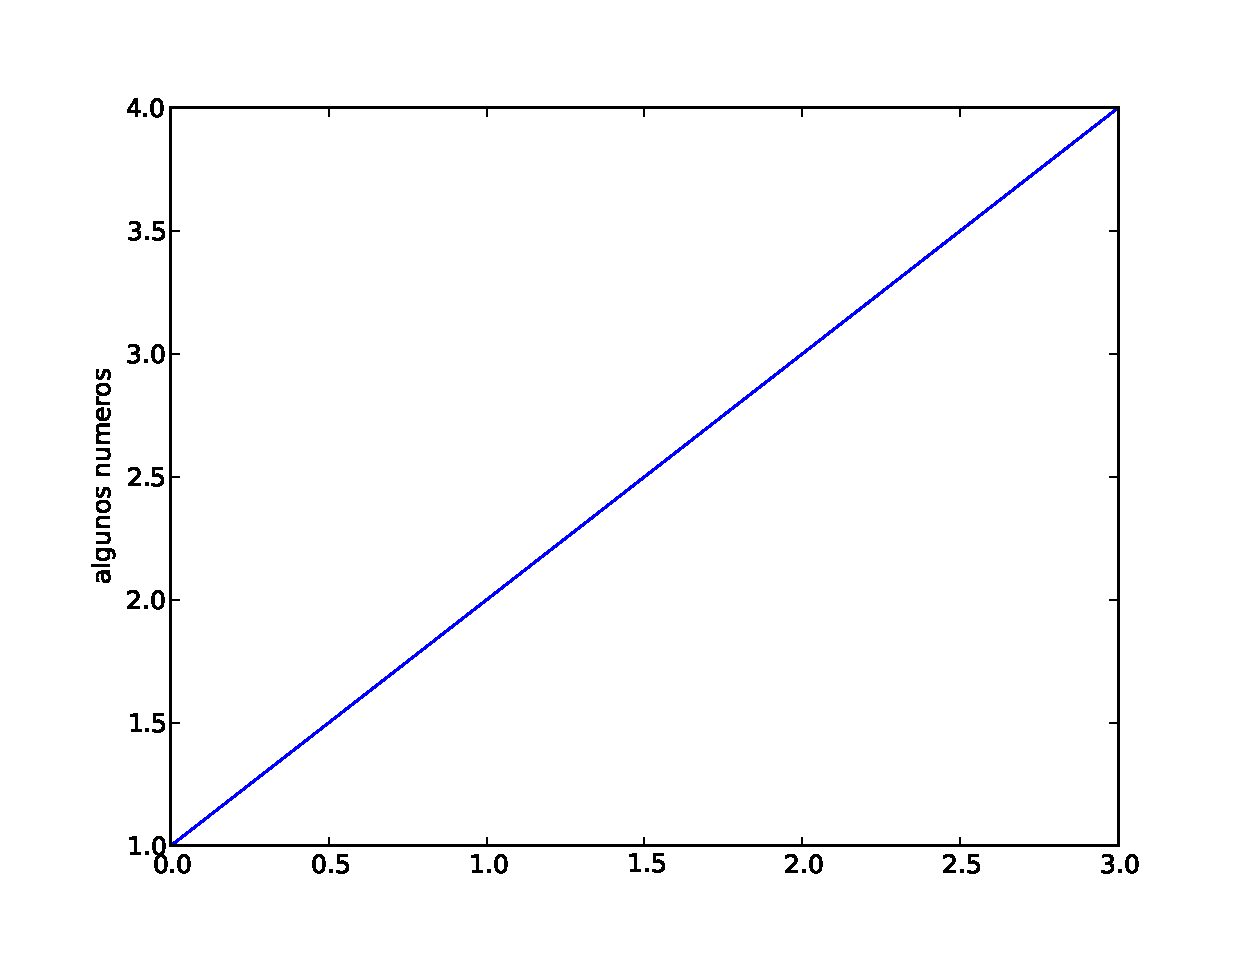
\includegraphics[scale=0.35]{plotEjercicio1.eps}<2> 
\end{figure}
\end{frame}
\begin{frame}
Te estarás preguntando por qué tenemos en el eje $x$ el rango $0-3$ y en el eje $y$ el rango  $1-4$.
\\
\medskip
\pause
Si proporcionamos una única lista o matriz en el comando \texttt{plot}, \texttt{matplotlib} asume que es una secuencia de valores de $y$, por lo que genera automáticamente los valores de $x$ para nosotros. Como los índices en \python comienzan en $0$, el vector $x$ por defecto tiene la misma longitud que $y$, pero inicia con 0. De ahí que los datos $x$ son $[0,1,2,3]$.
\end{frame}
\begin{frame}[fragile]
\frametitle{Ejecicio 2}
\begin{lstlisting}
import matplotlib.pyplot as plt
plt.plot([1,2,3,4], [1,4,9,16], 'ro')
plt.axis([0, 6, 0, 20])
plt.show()
\end{lstlisting}
\begin{figure}
	\centering
	\includegraphics[scale=0.35]{plotEjercicio2.eps}<2> 
\end{figure}
\end{frame}
\begin{frame}[fragile]
Por cada par $x$, $y$ de argumentos, existe un tercer argumento opcional, que es la cadena de formato que indica el color y tipo de línea.
\\
\medskip
Las letras y los símbolos de la cadena de formato son como en MATLAB, y concatenar una cadena de color con una cadena estilo de línea.
\\
\medskip
La cadena de formato por defecto es \verb|'b-'|, que es una línea de color azul.
\end{frame}
\begin{frame}[fragile]
\frametitle{Tipos de líneas}
\begin{tabular}{l | l}
carácter & descripción \\ \hline
\verb|'-'|	& línea sólida \\ \hline
\verb|'--'| & línea cortada \\ \hline
\verb|'-.'| & línea-punto \\ \hline
\verb|':'|	& línea de puntos \\ \hline
\verb|'.'|	& marca de punto \\ \hline
\verb|','|	& marca de pixel \\ \hline
\verb|'o'|	& marca de círculo \\ \hline
\verb|'v'|	& marca de triándulo hacia abajo \\ \hline
\verb|'^'|	& marca de triángulo hacia arriba
\end{tabular}
\end{frame}
\begin{frame}[fragile]
\frametitle{Lista de colores}
\begin{tabular}{l | l}
carácter & color \\ \hline
\verb|'b'| & azul \\ \hline
\verb|'g'| & verde \\ \hline
\verb|'r'| & rojo \\ \hline
\verb|'c'| & cyan \\ \hline
\verb|'m'| & magenta \\ \hline
\verb|'y'| & amarillo \\ \hline
\verb|'k'| & negro \\ \hline
\verb|'w'| & blanco
\end{tabular}
\end{frame}
\begin{frame}
\texttt{matplotlib} se limita a trabajar con listas, por lo que sería bastante acotado para el procesamiento y análisis numérico.
\\
\medskip
Por lo general, se utilizan los arreglos del módulo \texttt{numpy}. De hecho, todas las secuencias se convierten en matrices de \texttt{numpy} internamente.
\\
\medskip
El siguiente ejemplo ilustra un trazado de líneas con varios estilos diferentes en una sola instucción utilizando arreglos.
\end{frame}
\begin{frame}[fragile]
\frametitle{Ejecicio 3}
\begin{lstlisting}
import numpy as np
import matplotlib.pyplot as plt

t = np.arange(0., 5., 0.2)
plt.plot(t, t, 'r--', t, t**2, 'bs', t, t**3, 'g^')
plt.show()
\end{lstlisting}
\end{frame}
\begin{frame}[fragile]
\begin{figure}
	\centering
	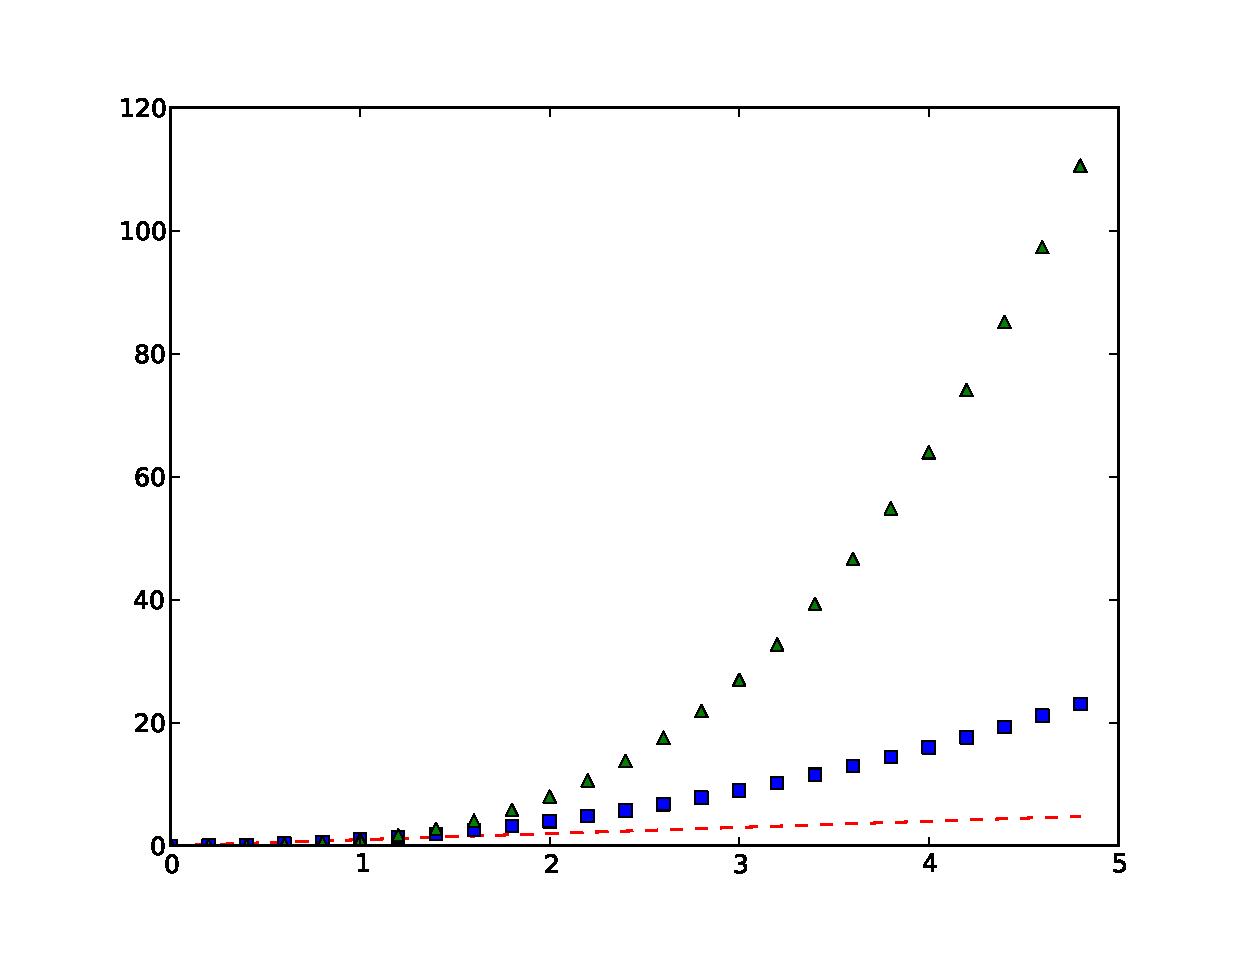
\includegraphics[scale=0.5]{plotEjercicio3.eps}
\end{figure}
\end{frame}
\begin{frame}[fragile]
\frametitle{Ejercicio 4}
Trabajando con múltiples gráficas
\begin{lstlisting}
import numpy as np
import matplotlib.pyplot as plt

def f(t):
    return np.exp(-t) * np.cos(2*np.pi*t)

t1 = np.arange(0.0, 5.0, 0.1)
t2 = np.arange(0.0, 5.0, 0.02)

plt.figure(1)
plt.subplot(211)
plt.plot(t1, f(t1), 'bo', t2, f(t2), 'k')

plt.subplot(212)
plt.plot(t2, np.cos(2*np.pi*t2), 'r--')
\end{lstlisting}
\end{frame}
\begin{frame}[fragile]
\begin{figure}
	\centering
	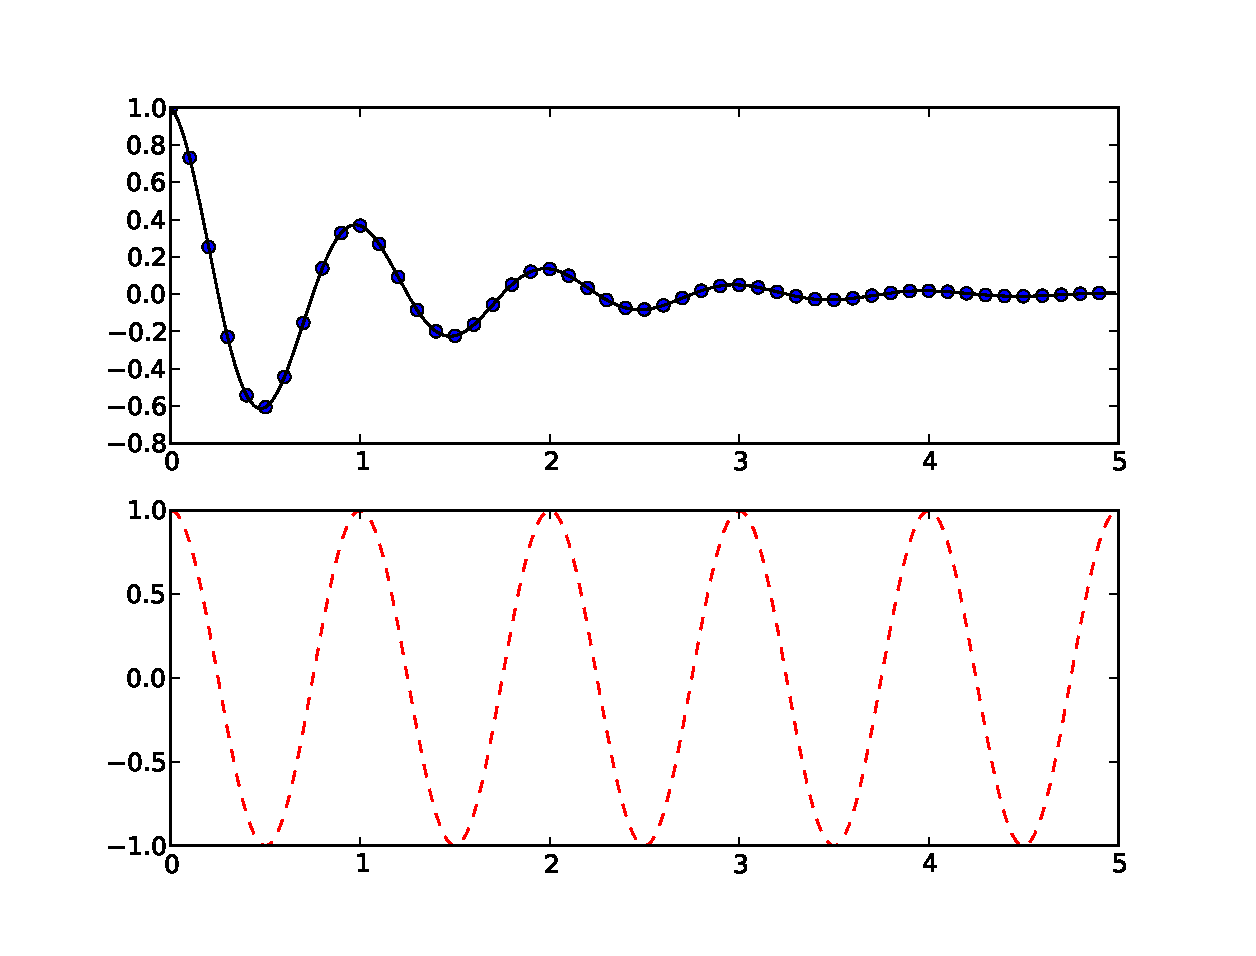
\includegraphics[scale=0.5]{plotEjercicio4.eps}
\end{figure}
\end{frame}
\begin{frame}
El comando \texttt{figure()} aquí es opcional, ya \texttt{figure(1)} se crea de forma predeterminada, así mismo \texttt{subplot(111)} se crea de forma predeterminada si no se especifica manualmente un eje.
\\
\medskip
El comando \texttt{subplot()} especifica \texttt{numrows, numcols, fignum} donde \texttt{fignum} varía en rango de 1 a \texttt{numrows * numcols}. Las comas en el comando \texttt{subplot()} son opcionales si \texttt{numrows * numcols} $<10$. Por tanto \texttt{subplot(211)} es idéntica a la \texttt{subplot(2,1,1)}.
\end{frame}
\begin{frame}[fragile]
\frametitle{Ejercicio 5}
\begin{lstlisting}
import matplotlib.pyplot as plt

plt.figure(1)                
plt.subplot(211)         
plt.plot([1,2,3])
plt.subplot(212)         
plt.plot([4,5,6])


plt.figure(2)                
plt.plot([4,5,6])           

plt.figure(1)                
plt.subplot(211)         
plt.title('Tan facil como 1,2,3')
plt.show()
\end{lstlisting}
\end{frame}
\begin{frame}[fragile]
\begin{figure}
	\centering
	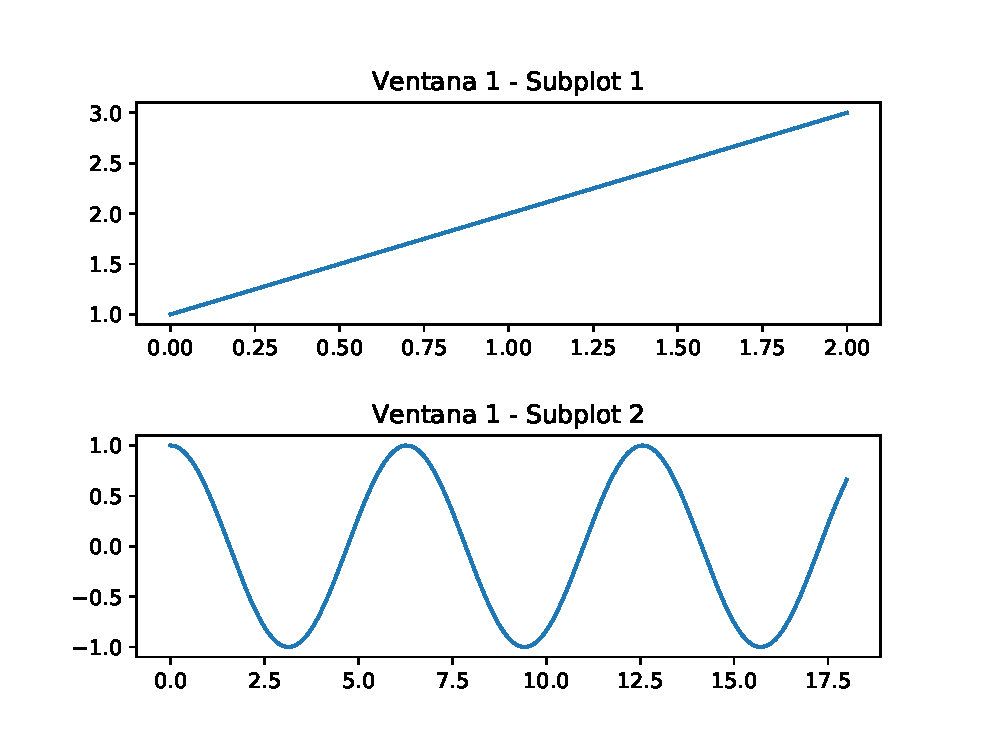
\includegraphics[scale=0.5]{plotEjercicio5_1.eps}<1>
	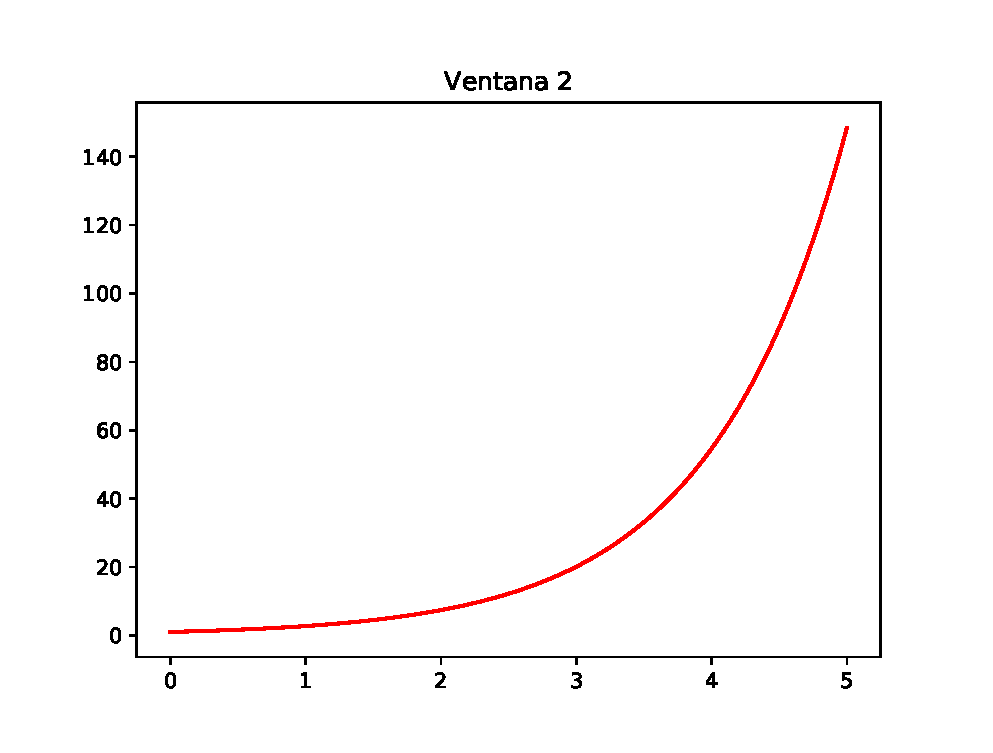
\includegraphics[scale=0.5]{plotEjercicio5_2.eps}<2>
\end{figure}
\end{frame}
\begin{frame}
\frametitle{Más recursos para graficar con \python}
Lo que hemos visto es una revisión muy básica y general de cómo generar una gráfica con \python, hay todavía una enorme cantidad de información sobre \texttt{matplotlib}, encontrarás en la página oficial de la librería, bastante documentación, ejemplos y elementos para extender completamente esta herramienta.
\\
\medskip
\pause
Se les proporcionará una guía breve de graficación, con la intención de que revisen casos prácticos aplicados a la física. Para cada gráfica que usemos más adelante en el curso, tendrán oportunidad de agregar más elementos que ustedes consideren.
\end{frame}
\section{Primeros problemas de la física}
\begin{frame}
\frametitle{Primeros problemas de la física}
De manera paralela a los conceptos importantes del curso, es necesario iniciar el trabajo de plantear algoritmos de solución a problemas de la física.
\\
\medskip
La mejor manera de aprender, es sentarse a programar. Debe de tenerse la calma para ello, la idea es ir perfeccionando las propuestas de solución, es importante señalar que la inspiración divina, no se da siempre.
\end{frame}
\begin{frame}[fragile]
\frametitle{Proceso de programación}
El proceso de programación consta de las actividades necesarias para escribir programas que funcionen adecuadamente como solución a un problema particular. \footnote{Amparo López Gaona, \textit{Introducción al desarrollo de programas con Java}, 3a. Ed., La Prensa de Ciencias, México D.F. 2013.}
\begin{enumerate}[<+->]
\item Definición del problema.
\item Diseño de la solución.
\item Codificación.
\item Depuración.
\item Mantenimiento.
\end{enumerate}
\end{frame}
\begin{frame}
\frametitle{Definición del problema}
Aquí se especifica qué es lo que debe de hacer el programa.
\\
\bigskip
Este primer paso puede parecer trivial aunque no lo es. La comprensión exacta de lo que se necesita hacer es requisito indispensable para crear una solución funcional.
\\
\medskip
En ocasiones, se ignora esta fase y se comienza a escribir un programa sin tener en claro el problema a resolver.
\end{frame}
\begin{frame}
\frametitle{Diseño de la solución}
En esta fase se indica una forma de satisfacer, mediante un programa, los requerimientos establecidos en la etapa anterior.
\\
\bigskip
El diseño de un programa es un proceso al que muchas veces no se le da la importancia y de ahí que en las etapas posteriores se tengan muchos problemas.
\\
\medskip
En el diseño es necesario identificar los principales componentes de la solución y la relación entre ellos.
\end{frame}
\begin{frame}
\frametitle{Codificación}
Una vez que se tiene el diseño de la solución, se procede a traducirlo a un lenguaje de programación.
\\
\bigskip
Esta tarea se conoce como codificación o implementación. En muchas ocasiones, uno se centra únicamente en esta etapa aunque, como se puede ver, el proceso de programar es mucho más complejo y creativo.
\end{frame}
\begin{frame}[fragile]
Es recomendable acostumbrarse desde el inicio a escribir programas que sean fácilmente entendibles por otras personas; podemos apoyarnos con lo siguiente:
\begin{enumerate}[<+->]
\item Los programas deben de tener una estructura clara.
\item El código debe estar organizado y presentado de manera que sea fácil su lectura.
\item El código debe de estar documentado.
\end{enumerate}
\end{frame}
\begin{frame}
\frametitle{Depuración}
El siguiente paso en el desarrollo de un programa es la depuración que consiste en verificar que el algoritmo y el programa sean adecuados. No importa que tan bonito esté el programa, si no produce los resultados deseados, simplemente no sirve.
\\
\bigskip
Depurar implica descubrir, localizar y corregir todos los errores que causen que un programa produzca resultados incorrectos o que no produzca ningún resultado.
\end{frame}
\begin{frame}
\frametitle{Mantenimiento}
En los programas y trabajos escolares, la tarea termina en el paso anterior, pero en la vida real no es así. La etapa de mantenimiento consiste en supervisar la operación de un programa, corregir cualquier error encontrado durante su uso continuo o efectuar modificaciones al mismo, con el propósito de que realice más tareas o de manera diferente a las que tenían contempladas originalmente.
\end{frame}
\subsection{Ejercicios de Mecánica}
\begin{frame}
\frametitle{Un primer problema de Mecánica}
Supongamos que tenemos una partícula de masa $m$ que está confinada a moverse a lo largo del eje $x$, bajo una fuerza $f(x)$. Sabemos de la ley de Newton que
\begin{equation}\label{Eqfuerza}
f = ma = m \dfrac{dv}{dt}
\end{equation}
donde $a$ es la aceleración y $v$ la velocidad de la partícula respectivamente, $t$ es el tiempo.
\\
\medskip
Si dividimos el tiempo en pequeños intervalos iguales $\tau = t_{i+1} - t_{i}$, sabemos que la velocidad en el tiempo $t_{i}$, está dada de manera aproximada por el promedio de la velocidad en el intervalo de tiempo $[t_{i}, t_{i+1}]$
\end{frame}
\begin{frame}
Por lo que
\begin{equation}\label{Eqvelocidad}
v_{i} \simeq \dfrac{x_{i+1}-x_{i}}{t_{i+1}-t_{i}} = \dfrac{x_{i+1}-x_{i}}{\tau}
\end{equation}
La aceleración de la partícula es aproximadamente el promedio de la aceleración en el mismo intervalo
\begin{equation}\label{Eqaceleracion}
a_{i} \simeq \dfrac{v_{i+1}-v_{i}}{t_{i+1}-t_{i}} = \dfrac{v_{i+1}-v_{i}}{\tau}
\end{equation}
donde $\tau$ es muy pequeño.
\end{frame}
\begin{frame}
El algoritmo más sencillo para determinar la posición y velocidad de la partícula en el tiempo $t_{1i+1}$, a partir de las cantidades correspondientes al tiempo $t_{i}$, se obtiene luego de combinar las ecuaciones (\ref{Eqfuerza}), (\ref{Eqvelocidad}) y (\ref{Eqaceleracion}), por lo que
\begin{eqnarray}
x_{i+1} &=& x_{i} + \tau v_{i} \label{Eqposicion} \\
v_{i+1} &=& v_{i} + \dfrac{\tau}{m} f_{i} \label{Eqvelocidadr}
\end{eqnarray}
donde $f_{i} = f(x_{i})$
\end{frame}
\begin{frame}
Si se proporciona la posición inicial y la velocidad de la partícula y se buscan las cantidades correspondientes en algún momento posterior (problema de valor inicial), podemos obtenerlas de forma recursiva a partir del algoritmo dado en las ecuaciones (\ref{Eqposicion}) y (\ref{Eqvelocidadr}).
\end{frame}
\subsection{Ejercicio 1: Oscilador mecánico}
\begin{frame}
\frametitle{Ejercicio 1: Oscilador mecánico}
Por simplicidad, consideremos que la fuerza es $f(x) = -kx$, donde $k$ es la constante del resorte. Usemos $m=k=1$. Queremos describir la posición y velocidad de la partícula en un intervalo de tiempo de 100 segundos. Las condiciones iniciales son las siguientes: $x(t=0) = 0$ y $v(t=0) = 1$.
\end{frame}
\begin{frame}[<+->]
\frametitle{Resolviendo el problema con Python}
¿Qué es lo que tenemos?
\begin{itemize}
\item El intervalo de tiempo de $[0,100]$ segundos.
\item La posición y velocidad inicial.
\item Las expresiones para calcular los $x_{i+1}$ y $v_{i+1}$
\end{itemize}
\visible<4->{¿Qué nos falta?}
\end{frame}
\begin{frame}[fragile]
\frametitle{Lo que nos falta}
\begin{itemize}[<+->]
\item Calcular para cada segundo en $[0,100]$ la posición y velocidad.
\item Guardar esos valores en un algún lado.
\item Graficar los resultados.
\end{itemize}
\end{frame}
\begin{frame}[fragile]
\frametitle{Uso de los módulos para nuestro programa}
Para graficar con el módulo \texttt{matplotlib} incluido en Python, necesitamos llamar a la librería \texttt{pyplot}, para acortar la escritura, usamos un \emph{alias}, en este caso \texttt{plt}.
\begin{lstlisting}
import matplotlib.pyplot as plt
from math import pi
\end{lstlisting}
\end{frame}
\begin{frame}[fragile]
\frametitle{Usando la información que nos proporciona el problema}
\begin{lstlisting}
n = 100

x = []
v = []

dt = 2* pi/n

x.append(0)
v.append(1)
\end{lstlisting}
\end{frame}
\begin{frame}[fragile]
\frametitle{Ciclo de iteración para los nuevos valores}
Como la fuerza en este caso es del tipo $f(x) = -kx$, tenemos un cambio de signo en el segundo sumando de $vi$.
\begin{lstlisting}
for i in range(n-1):
    xi = x[i] + v[i]*dt
    vi = v[i] - x[i]*dt
    
    x.append(xi)
    v.append(vi)
\end{lstlisting}
\end{frame}
\begin{frame}[fragile]
\frametitle{Generación de una gráfica}
La instrucción \texttt{plot}, nos permite crear en una nueva ventana, la gráfica, en este caso, requiere de una variable para poder desplegar los valores contenidos en la lista; el parámetro ''ro-'' lo usamos para decirle a matplotlib que nos devuelva una línea roja, con el símbolo ''o'', que estará ''unido'' entre sí por cada valor de la lista, además le agregamos una etiqueta para identificar nuestra gráfica. Hacemos lo mismo para la otra gráfica que nos representa la velocidad de la masa, ahora con color azul y el símbolo ''+''.
\begin{lstlisting}
plt.plot(x, "ro-", label="Posicion")
plt.plot(v, "b+-", label="Velocidad")
plt.legend(loc="upper right")
plt.xlabel("tiempo")
plt.show()
\end{lstlisting}
\end{frame}
\begin{frame}
\frametitle{Resultado del problema}
\begin{figure}
	\centering
	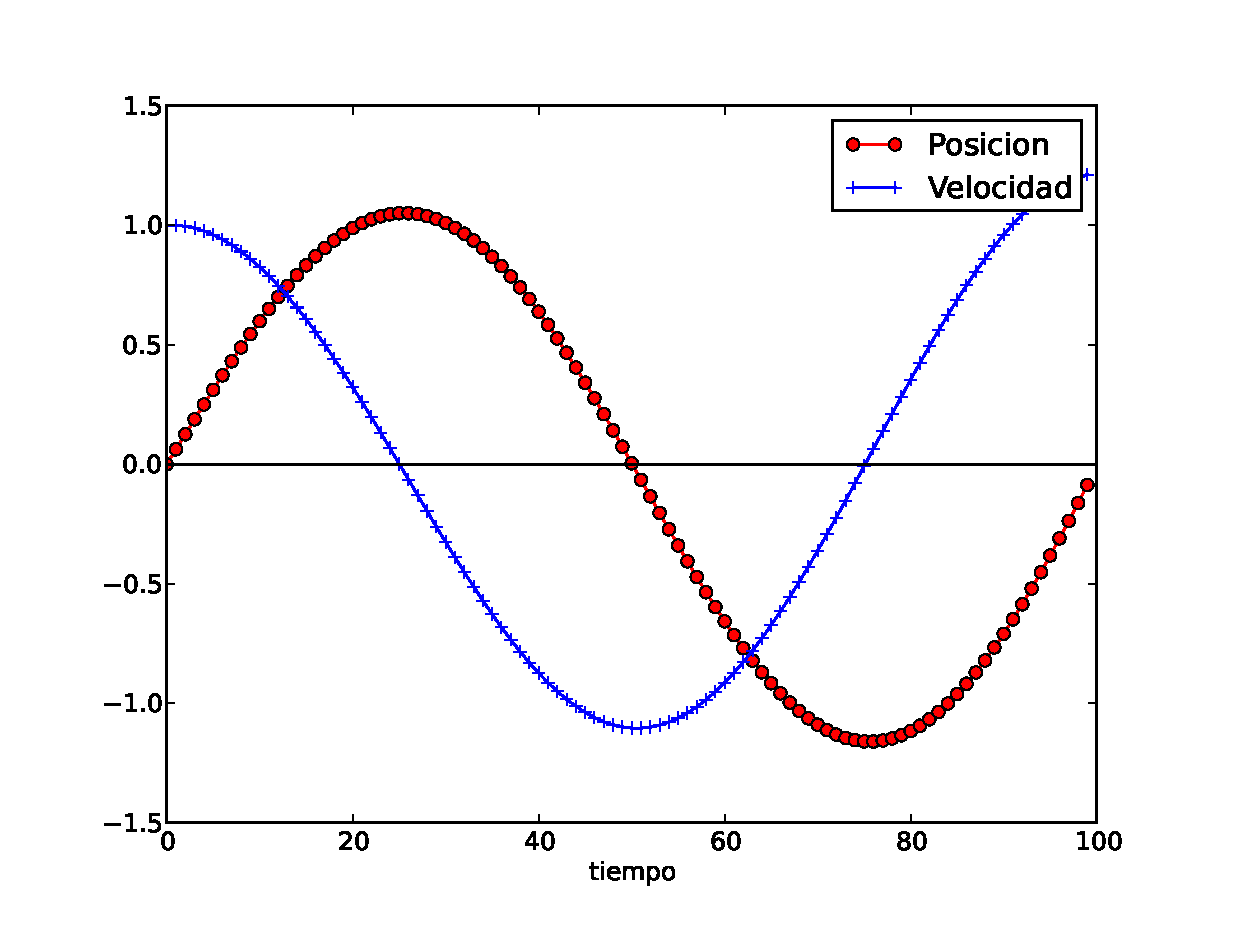
\includegraphics[scale=0.5]{Imagenes/EjerMecanica01.eps} 
\end{figure}
\end{frame}
\subsection{Ejercicio 2: Efecto de la resistencia del aire}
\begin{frame}
\frametitle{Ejecicio 2: Efecto de la resistencia del aire}
La bicicleta es una forma muy eficiente de transporte, este es un hecho bien conocido por cualquier persona que monta una. Nuestro objetivo en este ejercicio es comprender los factores que determinan la velocidad máxima de una bicicleta y estimar la velocidad de un caso real.
\\
\bigskip
Comenzaremos haciendo caso omiso de la fricción; tendremos que añadirlo al final, por supuesto, pero debemos primero entender cómo lidiar con el caso más simple y sin fricción.
\end{frame}
\begin{frame}
La ecuación de movimiento corresponde a la segunda ley de Newton, que escribimos de la forma
\begin{equation}\label{EqNewton2}
\dfrac{dv}{dt} = \dfrac{F}{m}
\end{equation}
donde $v$ es la velocidad, $m$ es la masa de la combinación de la bicicleta-conductor, $t$ es el tiempo, y $F$ es la fuerza en la bicicleta que viene del esfuerzo del conductor (en este caso vamos a suponer que la bicicleta se mueve sobre un terreno plano)
\end{frame}
\begin{frame}
Tratar correctamente a $F$ se complica por la mecánica de la bicicleta, ya que la fuerza ejercida por el ciclista se transmite a las ruedas por medio del plato, engranajes, cadena, etc. Esto hace que sea muy difícil derivar una expresión exacta para $F$.
\\
\medskip
Sin embargo, hay otra manera de abordar este problema que evita la necesidad de conocer la fuerza. Este enfoque alternativo implica la formulación del problema en términos de la potencia generada por el ciclista.
\\
\medskip
Estudios fisiológicos de ciclistas de carreras han demostrado que estos atletas son capaces de producir una potencia de salida de aproximadamente 400 watts durante largos períodos de tiempo ($\sim 1$ h)
\end{frame}
\begin{frame}
Usando las ideas de trabajo-energía podemos reescribir (\ref{EqNewton2}) como
\begin{equation}\label{EqPotencia}
\dfrac{dE}{dt} = P
\end{equation}
donde $E$ es la energía total, $P$ es la potencia de salida del ciclista. Para un trayecto plano la energía es totalmente cinética, es decir, $E = \frac{1}{2} m v^{2}$, y $\frac{dE}{dt} = mv (\frac{dv}{dt})$, usando esto en (\ref{EqPotencia}), resulta
\begin{equation}\label{EqPotenciavel}
\dfrac{dv}{dt} = \dfrac{P}{mv}
\end{equation}
\end{frame}
\begin{frame}
Si $P$ es una constante, la ecuación (\ref{EqPotenciavel}), se puede resolver de manera analítica, rearreglando términos:
\begin{equation}\label{EqIntegral}
\int_{v_{0}}^{v} v' dv' = \int_{0}^{t} \dfrac{P}{m} dt'
\end{equation}
donde $v_{0}$ es la velocidad de la bicicleta en $t=0$. Integrando ambos lados de la ecuación y resolviendo para $v$, tenemos
\begin{equation}\label{Eqvres}
v = \sqrt{v_{0}^{2} + 2 P \dfrac{t}{m}}
\end{equation}
\end{frame}
\begin{frame}[fragile]
\frametitle{Considera lo siguiente}
\begin{verbatim}
t = []
v = []

dt = 1

potencia = 400

masa = 70

tmax = 200

nmax = tmax/dt


t.append(0)
v.append(4)
\end{verbatim}
\end{frame}
\begin{frame}
\frametitle{Resultado de la velocidad sin fricción}
\begin{figure}
	\centering
	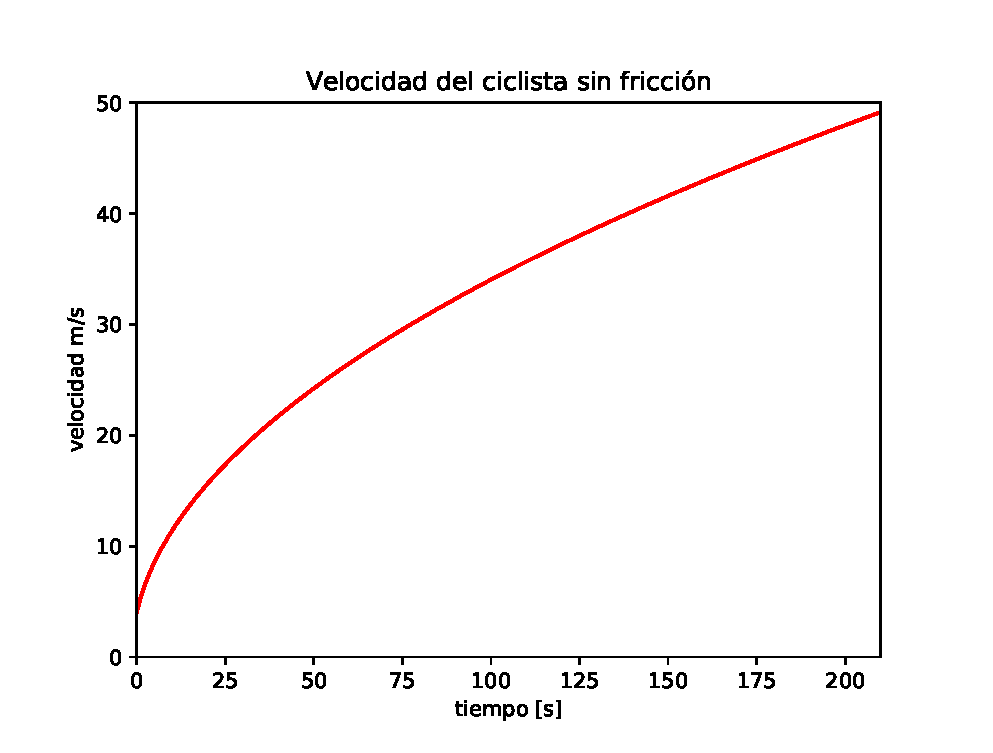
\includegraphics[scale=0.5]{EjerBicicleta01.eps}
\end{figure}
\end{frame}
\begin{frame}
Si bien esta es la solución correcta de la ecuación de movimiento (\ref{EqPotenciavel}), nuestro trabajo no concluye aquí, ya que predice que la velocidad se incrementará sin límite para tiempos muy largos.
\\
\medskip
Vamos a corregir este resultado, cuando se generaliza el modelo se debe de incluir el efecto de la resistencia del aire. El nuevo término que vamos a añadir a la ecuación de movimiento nos obliga a desarrollar una solución numérica, así que con eso en mente se considera un tratamiento numérico de (\ref{EqPotenciavel})
\end{frame}
\begin{frame}
Comenzamos con la forma de diferencias finitas para la derivada de la velocidad
\begin{equation}\label{Eqderivada}
\dfrac{dv}{dt} \simeq \dfrac{v_{i+1}-v_{i}}{\Delta t}
\end{equation}
donde asumimos que $\Delta t$ es paso discreto pequeño, y $v_{i}$ es la velocidad al tiempo $t_{i} \equiv i \Delta t$, por lo que de la ecuación (\ref{EqPotenciavel})
\begin{equation}\label{Eqveli+1}
v_{i+1} = v_{i} + \dfrac{P}{m v_{i}} \Delta t
\end{equation}
\end{frame}
\begin{frame}
Dada la velocidad en un tiempo $i$ (es decir, $v_{i}$), podemos usar (\ref{Eqveli+1}) para calcular un valor \textit{aproximado} de la velocidad en el siguiente paso $v_{i+1}$.
\\
\medskip
Si conocemos la velocidad inicial $v_{0}$, podemos obtener $v_{1}$, $v_{2}$, y así sucecivamente.
\end{frame}
\begin{frame}
\frametitle{Considerando la fricción del aire}
La fuerza debida a la fricción puede aproximarse de manera inicial como
\begin{equation}\label{EqFfriccion}
F_{a} \simeq - B_{1} v - B_{2} v^{2}
\end{equation}
Para velocidades muy bajas, el primer término es el que domina, y el coeficiente $B_{1}$ se puede calcular para objetos con formas sencillas.
\\
\medskip
Para una velocidad razonable $v^{2}$ el término domina sobre los demás, pero $B_{2}$ no puede calcularse exactamente en objetos sencillos como una pelota de beisbol, menos para una bicicleta.
\end{frame}
\begin{frame}
Podemos aproximar el valor de $B_{2}$ como sigue:
\\
\medskip
Si un objeto se mueve a través de la atmósfera y debe empujar fuera del camino el aire delante de él. La masa de aire movido en el tiempo $dt$ es $m_{aire} \sim \rho Avdt$, donde $\rho$ es la densidad del aire y $A$ el área frontal del objeto. A este aire se le da una velocidad de orden $v$, y por lo tanto, su energía cinética es $E_{aire} \sim m_{aire} v^{2} /2$
\\
\medskip
Este es también el trabajo realizado por la fuerza de arrastre (la fuerza sobre el objeto debido a la resistencia del aire) en el tiempo $dt$, por lo $F_{a}vdt = E_{aire}$. Poniendo todo esto junto nos encontramos
\[ F_{a} \simeq - C \rho A v^{2} \]
\end{frame}
\begin{frame}
Incluyendo este término en la expresión para la velocidad
\begin{equation}\label{Eqvelifriccion}
v_{i+1} = v_{i} + \dfrac{P}{m v_{i}} \Delta t - \dfrac{C \rho A v_{i}^{2}}{m} \Delta t
\end{equation}
Ahora te toca implementar el código, considerando $C = 0.5$ y $A=0.33$
\end{frame}
\begin{frame}
\frametitle{Comparando velocidades}
\begin{figure}
	\centering
	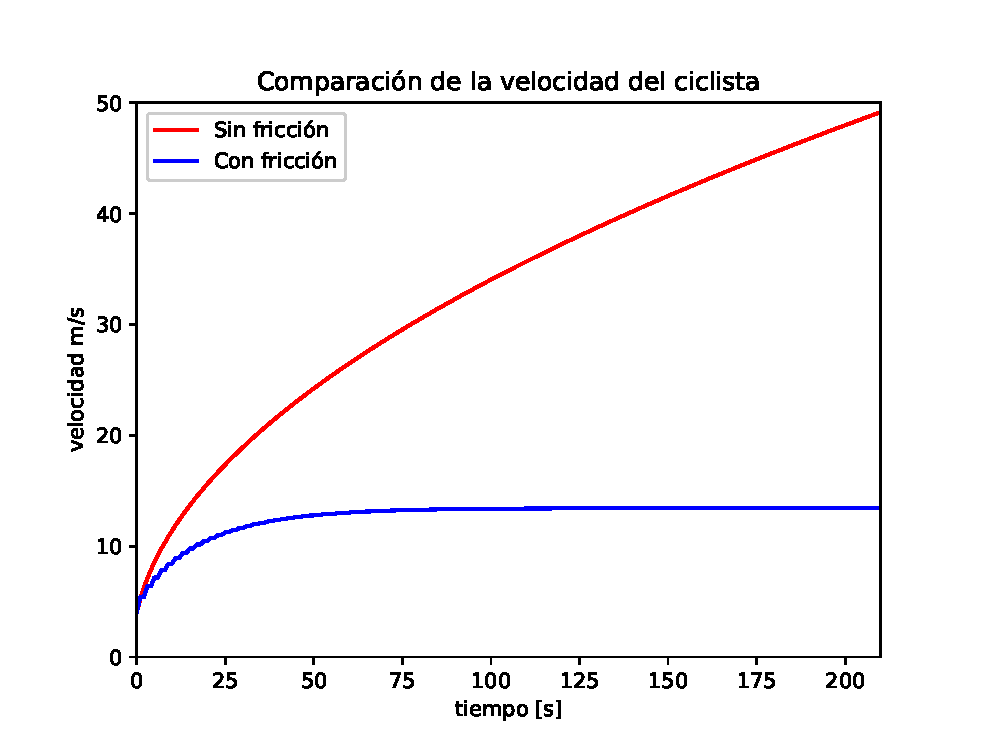
\includegraphics[scale=0.5]{EjerBicicleta02.eps}
\end{figure}
\end{frame}
\end{document}